% Created by tikzDevice version 0.12.3.1 on 2020-07-09 10:26:43
% !TEX encoding = UTF-8 Unicode
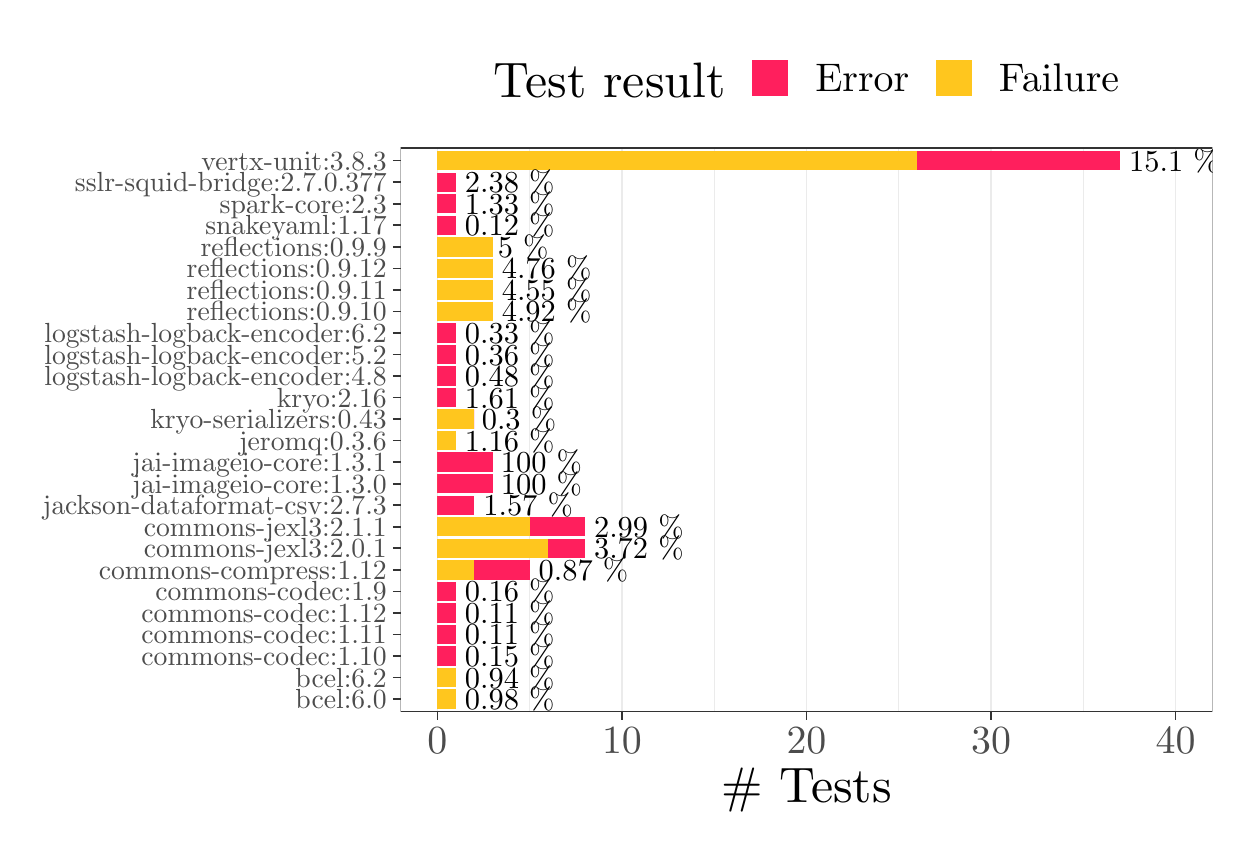
\begin{tikzpicture}[x=1pt,y=1pt]
\definecolor{fillColor}{RGB}{255,255,255}
\path[use as bounding box,fill=fillColor,fill opacity=0.00] (0,0) rectangle (433.62,289.08);
\begin{scope}
\path[clip] (  0.00,  0.00) rectangle (433.62,289.08);
\definecolor{drawColor}{RGB}{255,255,255}
\definecolor{fillColor}{RGB}{255,255,255}

\path[draw=drawColor,line width= 0.6pt,line join=round,line cap=round,fill=fillColor] (  0.00, -0.00) rectangle (433.62,289.08);
\end{scope}
\begin{scope}
\path[clip] (134.73, 41.81) rectangle (428.12,245.68);
\definecolor{fillColor}{RGB}{255,255,255}

\path[fill=fillColor] (134.73, 41.81) rectangle (428.12,245.68);
\definecolor{drawColor}{gray}{0.92}

\path[draw=drawColor,line width= 0.3pt,line join=round] (181.40, 41.81) --
	(181.40,245.68);

\path[draw=drawColor,line width= 0.3pt,line join=round] (248.08, 41.81) --
	(248.08,245.68);

\path[draw=drawColor,line width= 0.3pt,line join=round] (314.76, 41.81) --
	(314.76,245.68);

\path[draw=drawColor,line width= 0.3pt,line join=round] (381.44, 41.81) --
	(381.44,245.68);

\path[draw=drawColor,line width= 0.6pt,line join=round] (148.06, 41.81) --
	(148.06,245.68);

\path[draw=drawColor,line width= 0.6pt,line join=round] (214.74, 41.81) --
	(214.74,245.68);

\path[draw=drawColor,line width= 0.6pt,line join=round] (281.42, 41.81) --
	(281.42,245.68);

\path[draw=drawColor,line width= 0.6pt,line join=round] (348.10, 41.81) --
	(348.10,245.68);

\path[draw=drawColor,line width= 0.6pt,line join=round] (414.78, 41.81) --
	(414.78,245.68);
\definecolor{fillColor}{RGB}{255,31,93}

\path[fill=fillColor] (154.73, 42.98) rectangle (154.73, 49.98);

\path[fill=fillColor] (154.73, 50.76) rectangle (154.73, 57.76);

\path[fill=fillColor] (148.06, 58.54) rectangle (154.73, 65.55);

\path[fill=fillColor] (148.06, 66.32) rectangle (154.73, 73.33);

\path[fill=fillColor] (148.06, 74.11) rectangle (154.73, 81.11);

\path[fill=fillColor] (148.06, 81.89) rectangle (154.73, 88.89);

\path[fill=fillColor] (161.40, 89.67) rectangle (181.40, 96.67);

\path[fill=fillColor] (188.07, 97.45) rectangle (201.41,104.45);

\path[fill=fillColor] (181.40,105.23) rectangle (201.41,112.23);

\path[fill=fillColor] (148.06,113.01) rectangle (161.40,120.02);

\path[fill=fillColor] (148.06,120.79) rectangle (168.07,127.80);

\path[fill=fillColor] (148.06,128.57) rectangle (168.07,135.58);

\path[fill=fillColor] (154.73,136.36) rectangle (154.73,143.36);

\path[fill=fillColor] (161.40,144.14) rectangle (161.40,151.14);

\path[fill=fillColor] (148.06,151.92) rectangle (154.73,158.92);

\path[fill=fillColor] (148.06,159.70) rectangle (154.73,166.70);

\path[fill=fillColor] (148.06,167.48) rectangle (154.73,174.48);

\path[fill=fillColor] (148.06,175.26) rectangle (154.73,182.27);

\path[fill=fillColor] (168.07,183.04) rectangle (168.07,190.05);

\path[fill=fillColor] (168.07,190.83) rectangle (168.07,197.83);

\path[fill=fillColor] (168.07,198.61) rectangle (168.07,205.61);

\path[fill=fillColor] (168.07,206.39) rectangle (168.07,213.39);

\path[fill=fillColor] (148.06,214.17) rectangle (154.73,221.17);

\path[fill=fillColor] (148.06,221.95) rectangle (154.73,228.95);

\path[fill=fillColor] (148.06,229.73) rectangle (154.73,236.74);

\path[fill=fillColor] (321.43,237.51) rectangle (394.78,244.52);
\definecolor{fillColor}{RGB}{255,198,30}

\path[fill=fillColor] (148.06, 42.98) rectangle (154.73, 49.98);

\path[fill=fillColor] (148.06, 50.76) rectangle (154.73, 57.76);

\path[fill=fillColor] (148.06, 58.54) rectangle (148.06, 65.55);

\path[fill=fillColor] (148.06, 66.32) rectangle (148.06, 73.33);

\path[fill=fillColor] (148.06, 74.11) rectangle (148.06, 81.11);

\path[fill=fillColor] (148.06, 81.89) rectangle (148.06, 88.89);

\path[fill=fillColor] (148.06, 89.67) rectangle (161.40, 96.67);

\path[fill=fillColor] (148.06, 97.45) rectangle (188.07,104.45);

\path[fill=fillColor] (148.06,105.23) rectangle (181.40,112.23);

\path[fill=fillColor] (148.06,113.01) rectangle (148.06,120.02);

\path[fill=fillColor] (148.06,120.79) rectangle (148.06,127.80);

\path[fill=fillColor] (148.06,128.57) rectangle (148.06,135.58);

\path[fill=fillColor] (148.06,136.36) rectangle (154.73,143.36);

\path[fill=fillColor] (148.06,144.14) rectangle (161.40,151.14);

\path[fill=fillColor] (148.06,151.92) rectangle (148.06,158.92);

\path[fill=fillColor] (148.06,159.70) rectangle (148.06,166.70);

\path[fill=fillColor] (148.06,167.48) rectangle (148.06,174.48);

\path[fill=fillColor] (148.06,175.26) rectangle (148.06,182.27);

\path[fill=fillColor] (148.06,183.04) rectangle (168.07,190.05);

\path[fill=fillColor] (148.06,190.83) rectangle (168.07,197.83);

\path[fill=fillColor] (148.06,198.61) rectangle (168.07,205.61);

\path[fill=fillColor] (148.06,206.39) rectangle (168.07,213.39);

\path[fill=fillColor] (148.06,214.17) rectangle (148.06,221.17);

\path[fill=fillColor] (148.06,221.95) rectangle (148.06,228.95);

\path[fill=fillColor] (148.06,229.73) rectangle (148.06,236.74);

\path[fill=fillColor] (148.06,237.51) rectangle (321.43,244.52);
\definecolor{drawColor}{RGB}{0,0,0}

\node[text=drawColor,anchor=base west,inner sep=0pt, outer sep=0pt, scale=  1.10] at (164.65,112.71) {1.57 \%};

\node[text=drawColor,anchor=base west,inner sep=0pt, outer sep=0pt, scale=  1.10] at (157.98,151.62) {1.61 \%};

\node[text=drawColor,anchor=base west,inner sep=0pt, outer sep=0pt, scale=  1.10] at (157.98,229.43) {2.38 \%};

\node[text=drawColor,anchor=base west,inner sep=0pt, outer sep=0pt, scale=  1.10] at (157.98, 42.68) {0.98 \%};

\node[text=drawColor,anchor=base west,inner sep=0pt, outer sep=0pt, scale=  1.10] at (157.98, 50.46) {0.94 \%};

\node[text=drawColor,anchor=base west,inner sep=0pt, outer sep=0pt, scale=  1.10] at (157.98, 58.24) {0.15 \%};

\node[text=drawColor,anchor=base west,inner sep=0pt, outer sep=0pt, scale=  1.10] at (157.98, 73.81) {0.11 \%};

\node[text=drawColor,anchor=base west,inner sep=0pt, outer sep=0pt, scale=  1.10] at (157.98, 81.59) {0.16 \%};

\node[text=drawColor,anchor=base west,inner sep=0pt, outer sep=0pt, scale=  1.10] at (157.98, 66.02) {0.11 \%};

\node[text=drawColor,anchor=base west,inner sep=0pt, outer sep=0pt, scale=  1.10] at (184.65, 89.37) {0.87 \%};

\node[text=drawColor,anchor=base west,inner sep=0pt, outer sep=0pt, scale=  1.10] at (204.66,104.93) {2.99 \%};

\node[text=drawColor,anchor=base west,inner sep=0pt, outer sep=0pt, scale=  1.10] at (204.66, 97.15) {3.72 \%};

\node[text=drawColor,anchor=base west,inner sep=0pt, outer sep=0pt, scale=  1.10] at (157.98,213.87) {0.12 \%};

\node[text=drawColor,anchor=base west,inner sep=0pt, outer sep=0pt, scale=  1.10] at (171.01,128.27) {100 \%};

\node[text=drawColor,anchor=base west,inner sep=0pt, outer sep=0pt, scale=  1.10] at (171.01,120.49) {100 \%};

\node[text=drawColor,anchor=base west,inner sep=0pt, outer sep=0pt, scale=  1.10] at (157.98,159.40) {0.48 \%};

\node[text=drawColor,anchor=base west,inner sep=0pt, outer sep=0pt, scale=  1.10] at (157.98,174.96) {0.33 \%};

\node[text=drawColor,anchor=base west,inner sep=0pt, outer sep=0pt, scale=  1.10] at (157.98,167.18) {0.36 \%};

\node[text=drawColor,anchor=base west,inner sep=0pt, outer sep=0pt, scale=  1.10] at (164.10,143.84) {0.3 \%};

\node[text=drawColor,anchor=base west,inner sep=0pt, outer sep=0pt, scale=  1.10] at (157.98,221.65) {1.33 \%};

\node[text=drawColor,anchor=base west,inner sep=0pt, outer sep=0pt, scale=  1.10] at (171.32,182.74) {4.92 \%};

\node[text=drawColor,anchor=base west,inner sep=0pt, outer sep=0pt, scale=  1.10] at (171.32,190.53) {4.55 \%};

\node[text=drawColor,anchor=base west,inner sep=0pt, outer sep=0pt, scale=  1.10] at (169.91,206.09) {5 \%};

\node[text=drawColor,anchor=base west,inner sep=0pt, outer sep=0pt, scale=  1.10] at (171.32,198.31) {4.76 \%};

\node[text=drawColor,anchor=base west,inner sep=0pt, outer sep=0pt, scale=  1.10] at (398.03,237.21) {15.1 \%};

\node[text=drawColor,anchor=base west,inner sep=0pt, outer sep=0pt, scale=  1.10] at (157.98,136.06) {1.16 \%};
\definecolor{drawColor}{gray}{0.20}

\path[draw=drawColor,line width= 0.6pt,line join=round,line cap=round] (134.73, 41.81) rectangle (428.12,245.68);
\end{scope}
\begin{scope}
\path[clip] (  0.00,  0.00) rectangle (433.62,289.08);
\definecolor{drawColor}{gray}{0.30}

\node[text=drawColor,anchor=base east,inner sep=0pt, outer sep=0pt, scale=  1.00] at (129.78, 43.04) {bcel:6.0};

\node[text=drawColor,anchor=base east,inner sep=0pt, outer sep=0pt, scale=  1.00] at (129.78, 50.82) {bcel:6.2};

\node[text=drawColor,anchor=base east,inner sep=0pt, outer sep=0pt, scale=  1.00] at (129.78, 58.60) {commons-codec:1.10};

\node[text=drawColor,anchor=base east,inner sep=0pt, outer sep=0pt, scale=  1.00] at (129.78, 66.38) {commons-codec:1.11};

\node[text=drawColor,anchor=base east,inner sep=0pt, outer sep=0pt, scale=  1.00] at (129.78, 74.16) {commons-codec:1.12};

\node[text=drawColor,anchor=base east,inner sep=0pt, outer sep=0pt, scale=  1.00] at (129.78, 81.94) {commons-codec:1.9};

\node[text=drawColor,anchor=base east,inner sep=0pt, outer sep=0pt, scale=  1.00] at (129.78, 89.73) {commons-compress:1.12};

\node[text=drawColor,anchor=base east,inner sep=0pt, outer sep=0pt, scale=  1.00] at (129.78, 97.51) {commons-jexl3:2.0.1};

\node[text=drawColor,anchor=base east,inner sep=0pt, outer sep=0pt, scale=  1.00] at (129.78,105.29) {commons-jexl3:2.1.1};

\node[text=drawColor,anchor=base east,inner sep=0pt, outer sep=0pt, scale=  1.00] at (129.78,113.07) {jackson-dataformat-csv:2.7.3};

\node[text=drawColor,anchor=base east,inner sep=0pt, outer sep=0pt, scale=  1.00] at (129.78,120.85) {jai-imageio-core:1.3.0};

\node[text=drawColor,anchor=base east,inner sep=0pt, outer sep=0pt, scale=  1.00] at (129.78,128.63) {jai-imageio-core:1.3.1};

\node[text=drawColor,anchor=base east,inner sep=0pt, outer sep=0pt, scale=  1.00] at (129.78,136.41) {jeromq:0.3.6};

\node[text=drawColor,anchor=base east,inner sep=0pt, outer sep=0pt, scale=  1.00] at (129.78,144.20) {kryo-serializers:0.43};

\node[text=drawColor,anchor=base east,inner sep=0pt, outer sep=0pt, scale=  1.00] at (129.78,151.98) {kryo:2.16};

\node[text=drawColor,anchor=base east,inner sep=0pt, outer sep=0pt, scale=  1.00] at (129.78,159.76) {logstash-logback-encoder:4.8};

\node[text=drawColor,anchor=base east,inner sep=0pt, outer sep=0pt, scale=  1.00] at (129.78,167.54) {logstash-logback-encoder:5.2};

\node[text=drawColor,anchor=base east,inner sep=0pt, outer sep=0pt, scale=  1.00] at (129.78,175.32) {logstash-logback-encoder:6.2};

\node[text=drawColor,anchor=base east,inner sep=0pt, outer sep=0pt, scale=  1.00] at (129.78,183.10) {reflections:0.9.10};

\node[text=drawColor,anchor=base east,inner sep=0pt, outer sep=0pt, scale=  1.00] at (129.78,190.88) {reflections:0.9.11};

\node[text=drawColor,anchor=base east,inner sep=0pt, outer sep=0pt, scale=  1.00] at (129.78,198.66) {reflections:0.9.12};

\node[text=drawColor,anchor=base east,inner sep=0pt, outer sep=0pt, scale=  1.00] at (129.78,206.45) {reflections:0.9.9};

\node[text=drawColor,anchor=base east,inner sep=0pt, outer sep=0pt, scale=  1.00] at (129.78,214.23) {snakeyaml:1.17};

\node[text=drawColor,anchor=base east,inner sep=0pt, outer sep=0pt, scale=  1.00] at (129.78,222.01) {spark-core:2.3};

\node[text=drawColor,anchor=base east,inner sep=0pt, outer sep=0pt, scale=  1.00] at (129.78,229.79) {sslr-squid-bridge:2.7.0.377};

\node[text=drawColor,anchor=base east,inner sep=0pt, outer sep=0pt, scale=  1.00] at (129.78,237.57) {vertx-unit:3.8.3};
\end{scope}
\begin{scope}
\path[clip] (  0.00,  0.00) rectangle (433.62,289.08);
\definecolor{drawColor}{gray}{0.20}

\path[draw=drawColor,line width= 0.6pt,line join=round] (131.98, 46.48) --
	(134.73, 46.48);

\path[draw=drawColor,line width= 0.6pt,line join=round] (131.98, 54.26) --
	(134.73, 54.26);

\path[draw=drawColor,line width= 0.6pt,line join=round] (131.98, 62.04) --
	(134.73, 62.04);

\path[draw=drawColor,line width= 0.6pt,line join=round] (131.98, 69.83) --
	(134.73, 69.83);

\path[draw=drawColor,line width= 0.6pt,line join=round] (131.98, 77.61) --
	(134.73, 77.61);

\path[draw=drawColor,line width= 0.6pt,line join=round] (131.98, 85.39) --
	(134.73, 85.39);

\path[draw=drawColor,line width= 0.6pt,line join=round] (131.98, 93.17) --
	(134.73, 93.17);

\path[draw=drawColor,line width= 0.6pt,line join=round] (131.98,100.95) --
	(134.73,100.95);

\path[draw=drawColor,line width= 0.6pt,line join=round] (131.98,108.73) --
	(134.73,108.73);

\path[draw=drawColor,line width= 0.6pt,line join=round] (131.98,116.51) --
	(134.73,116.51);

\path[draw=drawColor,line width= 0.6pt,line join=round] (131.98,124.30) --
	(134.73,124.30);

\path[draw=drawColor,line width= 0.6pt,line join=round] (131.98,132.08) --
	(134.73,132.08);

\path[draw=drawColor,line width= 0.6pt,line join=round] (131.98,139.86) --
	(134.73,139.86);

\path[draw=drawColor,line width= 0.6pt,line join=round] (131.98,147.64) --
	(134.73,147.64);

\path[draw=drawColor,line width= 0.6pt,line join=round] (131.98,155.42) --
	(134.73,155.42);

\path[draw=drawColor,line width= 0.6pt,line join=round] (131.98,163.20) --
	(134.73,163.20);

\path[draw=drawColor,line width= 0.6pt,line join=round] (131.98,170.98) --
	(134.73,170.98);

\path[draw=drawColor,line width= 0.6pt,line join=round] (131.98,178.76) --
	(134.73,178.76);

\path[draw=drawColor,line width= 0.6pt,line join=round] (131.98,186.55) --
	(134.73,186.55);

\path[draw=drawColor,line width= 0.6pt,line join=round] (131.98,194.33) --
	(134.73,194.33);

\path[draw=drawColor,line width= 0.6pt,line join=round] (131.98,202.11) --
	(134.73,202.11);

\path[draw=drawColor,line width= 0.6pt,line join=round] (131.98,209.89) --
	(134.73,209.89);

\path[draw=drawColor,line width= 0.6pt,line join=round] (131.98,217.67) --
	(134.73,217.67);

\path[draw=drawColor,line width= 0.6pt,line join=round] (131.98,225.45) --
	(134.73,225.45);

\path[draw=drawColor,line width= 0.6pt,line join=round] (131.98,233.23) --
	(134.73,233.23);

\path[draw=drawColor,line width= 0.6pt,line join=round] (131.98,241.02) --
	(134.73,241.02);
\end{scope}
\begin{scope}
\path[clip] (  0.00,  0.00) rectangle (433.62,289.08);
\definecolor{drawColor}{gray}{0.20}

\path[draw=drawColor,line width= 0.6pt,line join=round] (148.06, 39.06) --
	(148.06, 41.81);

\path[draw=drawColor,line width= 0.6pt,line join=round] (214.74, 39.06) --
	(214.74, 41.81);

\path[draw=drawColor,line width= 0.6pt,line join=round] (281.42, 39.06) --
	(281.42, 41.81);

\path[draw=drawColor,line width= 0.6pt,line join=round] (348.10, 39.06) --
	(348.10, 41.81);

\path[draw=drawColor,line width= 0.6pt,line join=round] (414.78, 39.06) --
	(414.78, 41.81);
\end{scope}
\begin{scope}
\path[clip] (  0.00,  0.00) rectangle (433.62,289.08);
\definecolor{drawColor}{gray}{0.30}

\node[text=drawColor,anchor=base,inner sep=0pt, outer sep=0pt, scale=  1.44] at (148.06, 26.95) {0};

\node[text=drawColor,anchor=base,inner sep=0pt, outer sep=0pt, scale=  1.44] at (214.74, 26.95) {10};

\node[text=drawColor,anchor=base,inner sep=0pt, outer sep=0pt, scale=  1.44] at (281.42, 26.95) {20};

\node[text=drawColor,anchor=base,inner sep=0pt, outer sep=0pt, scale=  1.44] at (348.10, 26.95) {30};

\node[text=drawColor,anchor=base,inner sep=0pt, outer sep=0pt, scale=  1.44] at (414.78, 26.95) {40};
\end{scope}
\begin{scope}
\path[clip] (  0.00,  0.00) rectangle (433.62,289.08);
\definecolor{drawColor}{RGB}{0,0,0}

\node[text=drawColor,anchor=base,inner sep=0pt, outer sep=0pt, scale=  1.80] at (281.42,  9.00) {\# Tests};
\end{scope}
\begin{scope}
\path[clip] (  0.00,  0.00) rectangle (433.62,289.08);
\definecolor{fillColor}{RGB}{255,255,255}

\path[fill=fillColor] (162.93,256.68) rectangle (399.91,283.58);
\end{scope}
\begin{scope}
\path[clip] (  0.00,  0.00) rectangle (433.62,289.08);
\definecolor{drawColor}{RGB}{0,0,0}

\node[text=drawColor,anchor=base west,inner sep=0pt, outer sep=0pt, scale=  1.80] at (168.43,263.93) {Test result};
\end{scope}
\begin{scope}
\path[clip] (  0.00,  0.00) rectangle (433.62,289.08);
\definecolor{fillColor}{RGB}{255,255,255}

\path[fill=fillColor] (261.16,263.63) rectangle (275.62,278.08);
\end{scope}
\begin{scope}
\path[clip] (  0.00,  0.00) rectangle (433.62,289.08);
\definecolor{fillColor}{RGB}{255,31,93}

\path[fill=fillColor] (261.87,264.34) rectangle (274.91,277.37);
\end{scope}
\begin{scope}
\path[clip] (  0.00,  0.00) rectangle (433.62,289.08);
\definecolor{fillColor}{RGB}{255,255,255}

\path[fill=fillColor] (327.53,263.63) rectangle (341.98,278.08);
\end{scope}
\begin{scope}
\path[clip] (  0.00,  0.00) rectangle (433.62,289.08);
\definecolor{fillColor}{RGB}{255,198,30}

\path[fill=fillColor] (328.24,264.34) rectangle (341.27,277.37);
\end{scope}
\begin{scope}
\path[clip] (  0.00,  0.00) rectangle (433.62,289.08);
\definecolor{drawColor}{RGB}{0,0,0}

\node[text=drawColor,anchor=base west,inner sep=0pt, outer sep=0pt, scale=  1.44] at (284.62,265.89) {Error};
\end{scope}
\begin{scope}
\path[clip] (  0.00,  0.00) rectangle (433.62,289.08);
\definecolor{drawColor}{RGB}{0,0,0}

\node[text=drawColor,anchor=base west,inner sep=0pt, outer sep=0pt, scale=  1.44] at (350.98,265.89) {Failure};
\end{scope}
\end{tikzpicture}
